\documentclass{article}

\usepackage{tikz}
\usetikzlibrary{calc,arrows,decorations.pathmorphing,intersections}

\begin{document}

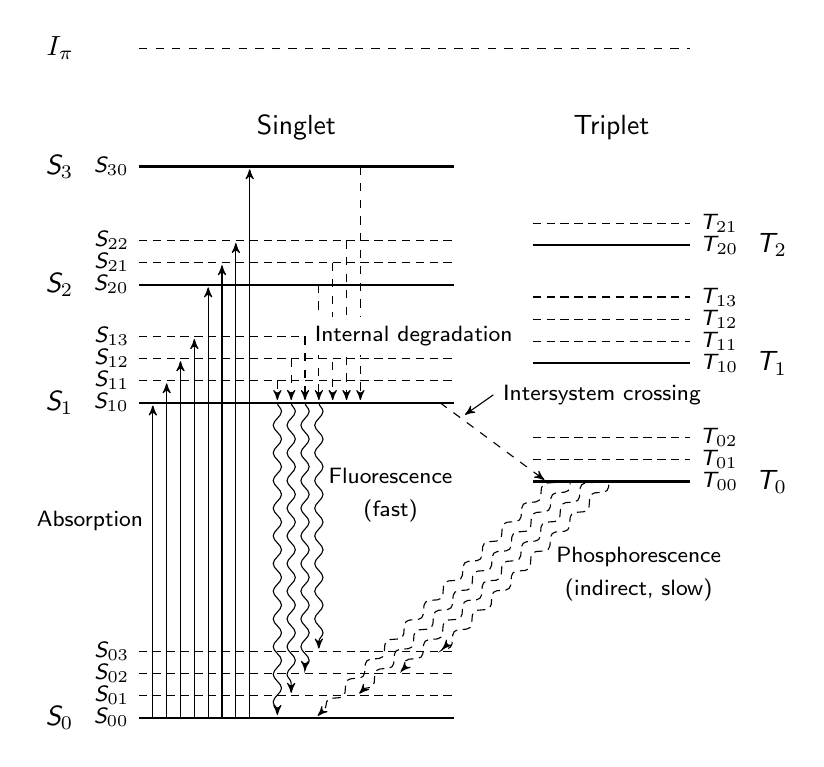
\begin{tikzpicture}[
 font=\sffamily,
 level/.style={black,thick},
 sublevel/.style={black,densely dashed},
 ionization/.style={black,dashed},
 transition/.style={black,->,>=stealth',shorten >=1pt},
 radiative/.style={transition,decorate,decoration={snake,amplitude=1.5}},
 indirectradiative/.style={radiative,densely dashed},
 nonradiative/.style={transition,dashed},
]
\coordinate (sublevel) at (0, 8pt);

% Singlet levels
\coordinate (S00) at (0, -1);
\coordinate (S01) at ($(S00) + (sublevel)$);
\coordinate (S02) at ($(S00) + 2*(sublevel)$);
\coordinate (S03) at ($(S00) + 3*(sublevel)$);
\coordinate (S10) at (0, 3);
\coordinate (S11) at ($(S10) + (sublevel)$);
\coordinate (S12) at ($(S10) + 2*(sublevel)$);
\coordinate (S13) at ($(S10) + 3*(sublevel)$);
\coordinate (S20) at (0, 4.5);
\coordinate (S21) at ($(S20) + (sublevel)$);
\coordinate (S22) at ($(S20) + 2*(sublevel)$);
\coordinate (S30) at (0, 6);

\foreach \level/\text in {00/0, 10/1, 20/2, 30/3}
    \draw[level] (S\level) node[left=20pt] {\itshape S$_\text$} node[left] {\footnotesize\itshape S$_{\level}$} -- +(4, 0);

\foreach \sublevel in {01,02,03,11,12,13,21,22}
    \draw[sublevel] (S\sublevel) node[left] {\footnotesize\itshape S$_{\sublevel}$} -- +(4, 0);

\node at (2, 6.5) {Singlet};

% Triplet levels
\coordinate (T00) at (5, 2);
\coordinate (T01) at ($(T00) + (sublevel)$);
\coordinate (T02) at ($(T00) + 2*(sublevel)$);
\coordinate (T03) at ($(T00) + 3*(sublevel)$);
\coordinate (T10) at (5, 3.5);
\coordinate (T11) at ($(T10) + (sublevel)$);
\coordinate (T12) at ($(T10) + 2*(sublevel)$);
\coordinate (T13) at ($(T10) + 3*(sublevel)$);
\coordinate (T20) at (5, 5);
\coordinate (T21) at ($(T20) + (sublevel)$);

\foreach \level/\text in {00/0, 10/1, 20/2}
    \draw[level] (T\level) -- +(2, 0) node[right=20pt] {\itshape T$_\text$} node[right] {\footnotesize\itshape T$_{\level}$};

\foreach \sublevel in {01,02,11,12,13,21}
    \draw[sublevel] (T\sublevel) -- +(2, 0) node[right] {\footnotesize\itshape T$_{\sublevel}$};

\node at (6, 6.5) {Triplet};

% Ionization
\draw[ionization] (0, 7.5) node[left=20pt] {$I_\pi$} -- +(7, 0);

% Excitations
\foreach \i/\from/\to in {1/S00/S10, 2/S00/S11, 3/S00/S12, 4/S00/S13, 5/S00/S20, 6/S00/S21, 7/S00/S22, 8/S00/S30}
    \draw[transition] ([xshift=\i*5pt] \from) -- ([xshift=\i*5pt] \to);

% Radiative decay (fluorescence)
\foreach \i/\from/\to in {1/S10/S00, 2/S10/S01, 3/S10/S02, 4/S10/S03}
    \draw[radiative] ([xshift=(\i+9)*5pt] \from) -- ([xshift=(\i+9)*5pt] \to);

% Nonradiative decay
\foreach \i/\from/\to in {1/S11/S10, 2/S12/S10, 3/S13/S10, 4/S20/S10, 5/S21/S10, 6/S22/S10, 7/S30/S10}
    \draw[nonradiative] ([xshift=(\i+9)*5pt] \from) -- ([xshift=(\i+9)*5pt] \to);

% Radiative decay (phosphorescence)
\begin{scope}
\clip (S00) -- +(7, 0) |- (T00) -| (S00);
\foreach \i/\level in {1/(S00), 2/(S01), 3/(S02), 4/(S03)} {
    \coordinate (Tstart) at ([xshift=\i*7pt] T00);
    \coordinate (end) at ($(Tstart) + (-135:4.5)$);
    \coordinate (start) at ($(Tstart)!-\i*5pt!(end)$);
    \path[name path=trans] (start) -- (end);
    \path[name path=ground] \level -- +(5, 0);
    \draw[indirectradiative,name intersections={of=trans and ground}] (start) --
        (intersection-1); }
\end{scope}

% Labels
\node[left] at (5pt, 1.5) {\footnotesize Absorption};
\node[right,align=center] at (13*5pt, 2cm - 5pt) {\footnotesize Fluorescence\\\footnotesize (fast)};
\node[right,align=center] at (5cm + 5pt, 1cm - 5pt) {
    \footnotesize Phosphorescence\\\footnotesize (indirect, slow)};
\node[right,fill=white,align=left] at ([xshift=12*5pt] S13) {\footnotesize Internal degradation};

% Intersystem crossing
\draw[nonradiative,name path=crossing] ($(S10) + (4, 0) - (5pt, 0)$) -- ([xshift=5pt] T00);
\coordinate (crosslabel) at (4.5, 3.1);
\node[right,fill=white] at (crosslabel) {\footnotesize Intersystem crossing};
\path[name path=arrow] (crosslabel) -- +(-145:1cm);
\draw[->,>=stealth',shorten >=2pt,name intersections={of=crossing and arrow}] (crosslabel) -- (intersection-1);

\end{tikzpicture}

\end{document}
